

\paragraph{Tipi di campionamento} Alcuni tipi di campionamento specifici:

\subparagraph*{Campionamento Stop-or-Go}
facciamo un campionamento ridotto, se trovo
ciò che cerco mi fermo (e.g. se i primi 20 elementi hanno zero errori allora mi fermo,
altrimenti...). Questo tipo di campionamento viene usato
quando l'IS auditor crede che relativamente pochi errori saranno
trovati nella popolazione.

\subparagraph*{Campionamento discovery:} usato quando
l'occorrenza dell'evento che sto cercando è molto rara.
È molto spesso usata quando lo scopo dell'audit è scoprire frodi,
infrazioni del regolamento o altre irregolarità.

\subparagraph*{Campionamento degli attributi:}
Un modello di campionamento usato per stimare la percentuale di
occorrenze di una specifica qualità (attributo) all'interno della
popolazione. Un \textbf{attributo} è qualsiasi
caratteristica che identifica una transazione rispetto alle altre (es.
transazioni effettuate ad un certo orario).\\
\textbf{Tasso di errore tollerabile:} il massimo rate di errore
tollerabile prima di dichiarare che l'affermazione da verificare
sia falsa.\\


\subparagraph*{Campionamento variabile}
Viene usato per capire quanto è accurato il campione nel rappresentare
l'intera popolazione. Questo campionamento si può riferire
a diversi tipi di modelli di campionamento quantitativo:


\begin{figure}[h!]
        \begin{center}
                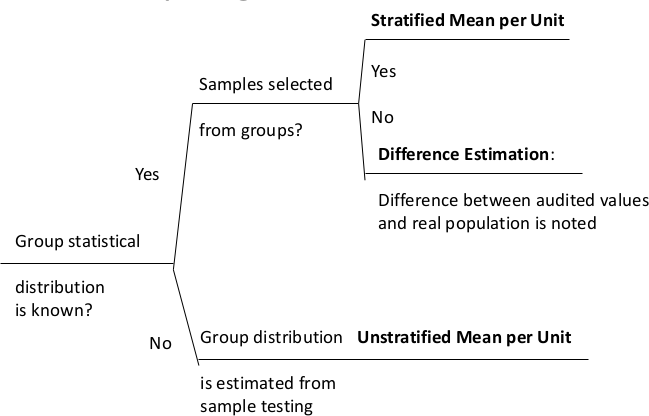
\includegraphics[scale=0.5]{res/img/variable_sampling.png}
        \end{center}
        \caption{Procedimento per il campionamento variabile.}
        \label{fig:variable:sampling}
\end{figure}

\begin{itemize}
\item \textbf{Stratified mean per unit:}
Modello di campionamento statistico in cui la popolazione
viene divisa in gruppi e i campioni sono estratti dai vari
gruppi. È usato per produrre dimensioni dei campioni più piccoli
dell'\textit{unstratified mean per unit}.

\item \textbf{Unstratified mean per unit:}
Modello di campionamento statistico in cui viene calcolato la media
del campione e usato come stima del totale.


\item \textbf{Difference Estimation Sampling:} Un modello statistico
usato per stimare la differenza totale
tra i valori auditati e i valori non auditati dichiarati ottenuti
dalle osservazioni del campione.

Problemi tipici che bisogna indirizzare sono la media e la deviazione standard.
La \textbf{media} non è un fenomeno che cattura bene l'andamento generale, per la
presenza di \textit{outlier}, ovvero dei punti fuori dal comportamento
tipico del campione.
La media è un parametro poco affidabile (va verificato ulteriormente). Un
parametro più affidabile che non è soggetto agli
outlier è la \textbf{mediana}.
\end{itemize}

La loro relazione è riportata nella Figura~\ref{fig:variable:sampling}.


\paragraph*{Ultime considerazioni}
Un problema è la possibilità di usare una
distribuzione fallace completamente duale rispetto all'intervallo di
confidenza.



\subsection{Step 8: Preparare il rapporto di Audit}

È importante identificare:
\begin{itemize}
\item Chi deve ricevere il rapporto?
\item Contesto (cosa viene analizzato), gli obiettivi, il periodo coperto e
quanto l'audit è durato\footnote{Audit che durano troppo poco con tante persone
da analizzare non vanno bene, soprattutto se devono essere svolti in poco
tempo.};
\item Findings (quello che è stato trovato), che deve essere supportato da delle
\emph{evidence} (prove). Le raccomandazioni possono essere date in due modi:
seguendo gli standard (es. standard ISO) o mettendo assieme la nostra
esperienza, la nostra conoscenza e quello che può fare l'azienda per risolvere i
problemi evidenziati;
\item Raggruppare per concretezza delle evidenze che abbiamo trovato;
\item Menzionare i problemi trovati e le critiche costruttive.
\end{itemize}

Il rapporto di audit è una parte molto importante: un rapporto dettagliato
permette ai successori di verificare il corretto funzionamento o meno
dell'azienda negli anni passati e permette di capire meglio il contesto. Un
rapporto di audit dovrebbe essere bilanciato, altrimenti se si arriva a mettere
a fuoco troppe cose negative non va bene, ma è importante anche non trascurarle.
È importante tenere a mente che il rapporto di audit è fatto per essere letto
dai ``piani alti''. Tenersi alle prove e ai fatti è sempre un'azione
consigliata.

\subsubsection{Evidenza}

Sono delle prove e esistono in diverse forme: note dalle interviste, risultati
dei test, email o corrispondenza, documentazione e osservazioni.

Le migliori fonti per ottenere informazioni sono:
\begin{itemize}
\item \textbf{Esterne:} fonti da organizzazioni esterne (es. i fornitori);
\item \textbf{Qualificate:} le più autorevoli;
\item \textbf{Oggettive:} evidenze per cui non è possibile esprimere un
parere soggettivo
\item \textbf{Tempo:} deve essere coerente con il periodo della nostra attività
di audit
\end{itemize}

\subsubsection{Comunicazione dei risultati}

La comunicazione dei risultati è un passo decisivo. Questi risultati devono
essere riportati alle persone interessate. Queste sono:
\begin{itemize}
  \item ai manager di basso livello deve essere riportato il materiale
  riguardante la loro area di interesse e dove l'auditor e il manager si
  trovando di comune accordo su un problema, devono essere sviluppati dei corsi
  per correggerlo, mentre invece dove c'è un disaccordo devono essere spiegate
  le conseguenze a cui un problema può portare.
  \item ai manager di alto livello invece deve essere consegnata la parte più
  grossa, con tutti i ritrovamenti di interesse dell'audit.
\end{itemize}
Ciò è schematizzato nella Figura~\ref{fig:consegnarisultati}

\begin{figure}[h!]
        \begin{center}
                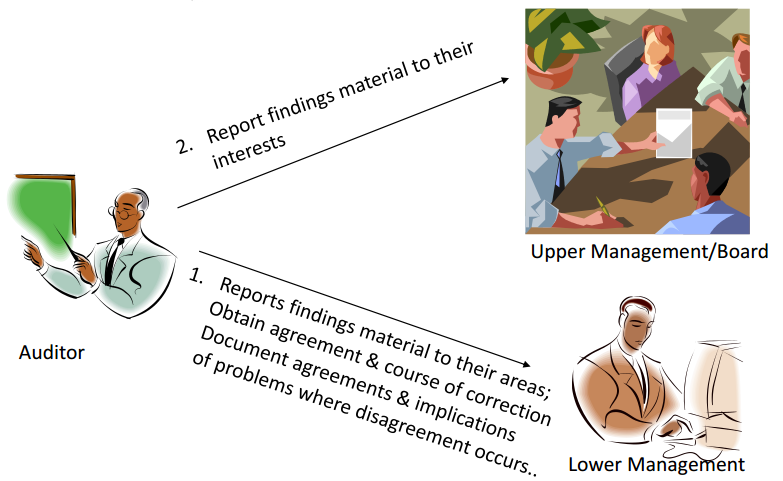
\includegraphics[scale=0.4]{res/img/communication_audit.png}
        \end{center}
        \caption{Procedimento per la comunicazione dei risultati dell'audit.}
        \label{fig:consegnarisultati}
\end{figure}

\subsection{Step 9: Prosieguo}


Il \textit{follow-up} serve a verificare se il management ha intrapreso le azioni
necessarie a correggere i problemi in tempo.

Dopo aver consegnato il report dell'audit, l'auditor deve condurre
delle interviste d'uscita con il management per ottenere il suo
impegno per implementare le raccomandazioni contenute nel report.
Dopo aver preso nota delle raccomandazioni, il management deve
indicare le azioni correttive che vuole implementare e una data
approssimativa per l'implementazione.

È compito dell'auditor -- nei successivi audit --
controllare che il management abbia onorato
i propri impegni nel sistemare o rimediare a deficienze trovate negli
audit precedenti.
Alcuni problemi non vengono corretti perchè cambiamenti nella pratica o
nel design organizattivo hanno già eliminato le debolezze riscontrate nei
controlli precedenti.

\section{Raccomandazioni finali sull'Audit}

Queste ultime note sono molto importanti e vanno sempre tenute in
considerazione:
\begin{itemize}
\item Mai eccedere lo scopo di quello che si deve fare, ovvero mai ficcare il
naso dove non serve. I permessi che vengono accordati devono essere messi per
iscritto, affinché ne rimanga una traccia.
\item Tutti i test potrebbero impattare sul sistema quindi è una buona
pratica avvisare i settori interessati dei possibili disservizi prima di eseguire
qualsiasi test.
\item Quando si lavora con i dati è importante non toccare dati o configurazioni
importanti.
\end{itemize}


\section{Tipi di audit}

Gli audit possono essere classificati in varie tipologie:
\begin{itemize}
\item \textbf{Audit finanziario}: assicura l'integrità degli asset
finanziari;
\item \textbf{Audit operazionale}: valuta i controlli interni per uno
specifico processo/area;
\item \textbf{Audit integrativo}: include sia aspetti finanziari
che operazionali;
\item \textbf{Audit forense}: è successo un evento negativo che ha
scatenato reazioni civili o penali e viene chiamato un auditor
esterno per fare analisi forense;
\item \textbf{Audit IS}: verifica che l'IS stia salvaguardando i dati
e che stia fornendo CIA in modo efficiente;
\item \textbf{Audit amministrativo}: verifica l'efficienza dei processi
e dell'organizzazione.
\end{itemize}


\subsection{Computer-Assisted Audit Techniques (CAAT)}
Durante il corso di un audit, l'auditor deve cercare di raccogliere
prove rilevanti e utili per raggiungere gli obiettivi dell'audit.
I finding e le conclusioni dell'audit devono essere supportate da 
analisi appropriate e interpretazione delle prove.

I CAAT sono strumenti importanti per l'auditor per raccogliere
informazioni dagli ambienti di processing dell'informazione.
In particolar modo quando i sistemi hanno hardware, software, strutture
dati e formati di record differenti, è quasi imposibile per un auditor
raccogliere le prove senza un tool.

Questi software permettono agli auditor di:
\begin{itemize}
\item Accedere e analizzare i dati nel database;
\item Effettuare test di conformità;
\item Effettuare penetration test;
\item Testare le applicazioni.
\end{itemize}

I CAAT includono diversi tipi di tool e tecniche come per esempio
i generalized audit software (GAS), software di utility e
software di debbugging e scanning.

\subsubsection{Generalized Audit Software (GAS)}
Il termine GAS si riferisce a software standard capaci di leggere
ed accedere a dati da diversi database, flat-file e file in formato
ASCII. Gli IS auditor possono usare i GAS per analizzare indipendentemente
i dati e usare software di alto livello per invocare delle funzioni
sui file contenenti i dati.

Questa tipologia di tool sono molto utili e permettono agli auditor di:
\begin{itemize}
\item Avere accesso ai file: leggere i record e la struttura del file;
\item Riorganizzare i file: permettono l'indexing, l'ordinamento,
il merging e la creazione di link ad altri file;
\item Selezionare dei dati: selezionare un insieme di record,
applicazione di filtri, ecc\dots;
\item Eseguire funzioni statistiche: permettono il campionamento, 
la stratificazione e l'analisi della frequenza;
\item Eseguire Funzioni aritmetiche: permettono di eseguire operazioni e 
funzioni matematiche sui dati contenuti nei file.
\end{itemize}



\subsection{Autovalutazione del controllo}

Sistema di audit interno che migliora l'audit esterno. I benefici consistono
nel fatto che si lavora con le persone e questo serve per insegnare ai
dipendenti e dare una migliore immagine dell'azienda.


\subsection{Service Learning Component: Non-Disclosure Agreement}

Supponiamo che si sia una situazione del genere:

\begin{verbatim}
You: I developed an audit plan for Help-The-Community
Interviewer: What specifically did you do?
You: We tried to break into their wireless network
Interviewer: What did you find?
You: They had no security. They were hopelessly non-technical.
Their password was `HelpTheCommunity', and transmissions were
unencrypted. I could read everything...
\end{verbatim}

In questo dialogo, è evidente come ci sia un rilascio di informazioni non
controllato, che potrebbe portare un attacco di tipo malizioso.

Il problema è che l'intervistato ha divulgato informazioni sull'azienda,
nonostante il NDA. Anche se i problemi fossero attualmente risolti sta comunque
infangando il nome della società sotto audit.


Un comportamento corretto potrebbe essere:
\begin{verbatim}
You: I developed an audit plan for Help-The-Community
Interviewer: What specifically did you do?
You: We did a penetration test. However, I signed a
non-disclosure agreement, so I am not at liberty to
say specifically what we did or found.
Interviewer: Were you successful in breaking in?
You: I can't say. However, if you would like to contact my
community partner as a reference, here is her contact
information...
\end{verbatim}

\section{Esercizi}
Gli esercizi su questa parte si trovano in \ref{EsAudit}.

%ESERCIZI

% Ho lasciato qui i commenti degli esercizi perché c'è una nota che non so dove
% posizionarla, quindi così riusciamo a capire che numero di esercizio è riferito
% quella nota contando il numero di ``Altro esercizio'' qui scritti!

% Altro esercizio



% Altro esercizio


%Altro esercizio


%Altro esercizio

%Altro esercizio

%Altro esercizio

%Altro esercizio

% RISCHIO DI CONTROLLO = QUANDO IL CONTROLLO FALLISCE -> Per mitigarlo si usano
% controlli compensativi

%Altro esercizio

%Altro esercizio
